\section{Misalignment Studies} \label{sec:misalign}

In order to protect both the active area of the SiPMs and the scintillator surface at the upstream end, a small air gap was necessary between these two surfaces.  Similarly, during assembly the scintillator paddles were also shimmed radially such that the top edge of the scintillator was level with the top edge of the active area of the SiPM thereby maximizing light collection.  In this section we discuss the relative alignment of a machined scintillator paddle and a SiPM readout detector array and its effects on light collection and time resolution.

\subsection{Experimental Set-up} \label{sec:misalign_setup}
% WB this needs to be shortened and summarized. You can make references to your thesis for all the details.
% EP done.

A custom fabricated test stand, further discussed in Sec.~\ref{sec:fab_test}, and a polished scintillator machined to the nominal ST geometry, were utilized for the misalignment studies.  The readout SiPM sat atop a Newport MT-XYZ (MT) compact dovetail XYZ linear translation stage\cite{newport_mt_xyz} with three fine adjustment screws consisting of 80 threads per inch.  Each knob for the three axes provides a translation of $318\ \mathrm{\mu m}$ per rotation.  For each location of the SiPM, the source and trigger PMT were located $\mathrm{24.5~cm}$ downstream from the readout end. 

%To study the effects of the various horizontal (translations along the $z-axis$) coupling distances, the relative position of the active area of the SiPM and the top edge of the scintillator paddle, or vertical (translations along the $y-ais$) alignment, was required to be known prior too.

Utilizing an Edmund Optics complementary metal oxide semiconductor (CMOS) camera, both the vertical and horizontal alignment (coupling distance) of the active area of the SiPM and scintillator was measured with $25~\mathrm{\mu m}$ accuracy.
% WB make this schematical, the photos are no clear.
% EP done.
	\begin{figure}[!htb]
		\centering
		%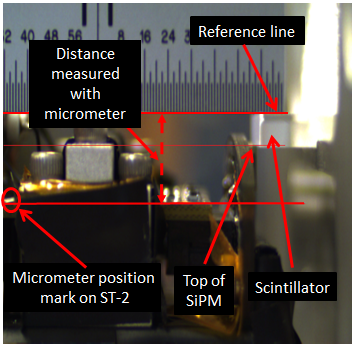
\includegraphics[width=0.8\columnwidth]{misalignment/figs/sipm_va_optics}
		%\caption{Vertical alignment optics set-up.  The reference line corresponds to the top surface of the scintillator, while the micrometer position on the ST2 is clearly marked so that the absolute difference could be measured both optically and manually with a micrometer.}
		%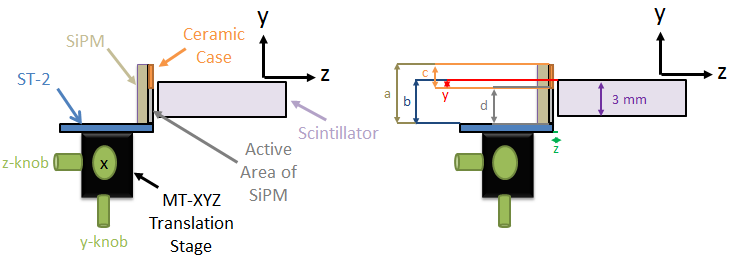
\includegraphics[width=1.0\columnwidth]{misalignment/figs/sipm_va_optics_schematic}
		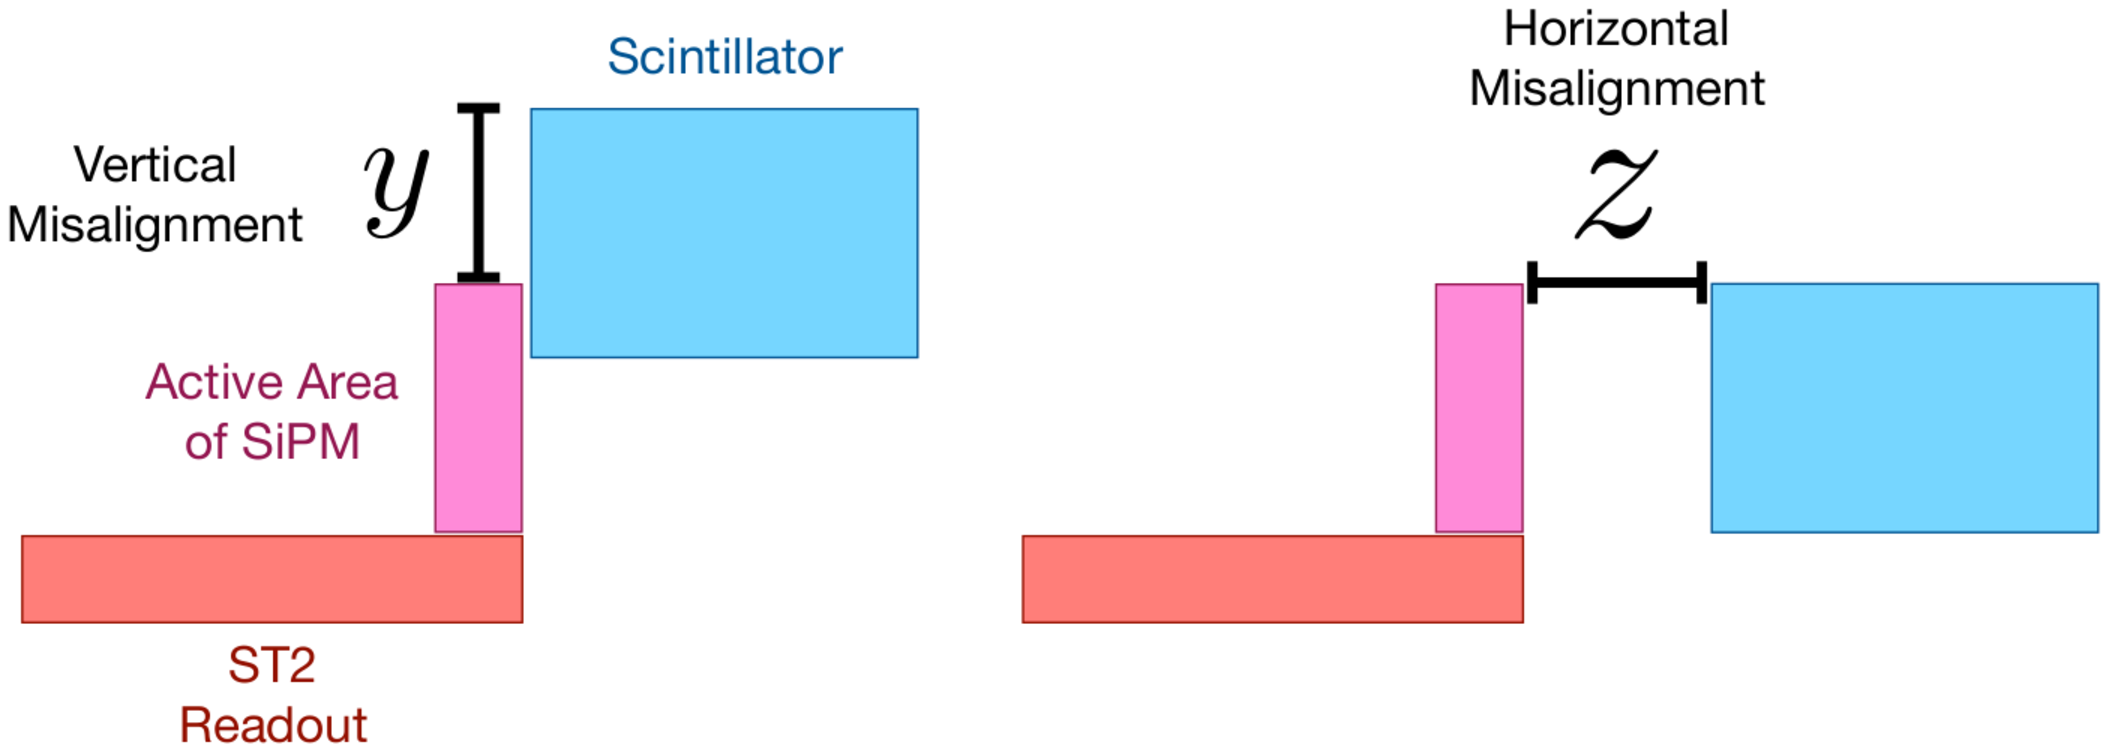
\includegraphics[width=1.0\columnwidth]{misalignment/figs/st_misalignment}
		\caption{Optics setup for misalignment studies.  Left: SiPM \& scintillator vertical misalignment. Right: SiPM \& scintillator horizontal misalignment}
		\label{fig:sipm_va_optics}
	\end{figure}
A micrometer, with $25~\mathrm{\mu m}$ resolution, was utilized in order to cross check the optical measurements and to provide absolute measurements of fixed distances in the experimental set-up. Further details of the experimental set-up are discussed in Ref.~\cite{pooser16}.

\subsection{Vertical Alignment of SiPM \& Scintillator}
\label{sec:misalign_vert}

% WB make the text shorter, basically just describe the result an compare to simulations. 
% EP done.
% WB The scales in Fig. 19 and 18 should be similar in order to compare simulation to measurement.
% EP the scales cannot be made similar since the simulation data no longer exists.

In order to measure the time resolution at various vertical alignment configurations, the scintillator remained fixed while the SiPM scanned across the upstream end of the scintillator ($y$) as can be seen in the left of Fig.~\ref{fig:sipm_va_optics}. The coupling distance between the active area of the SiPM and scintillator ($z$) remained at a constant distance of $\mathrm{100\ \mu m}$ and was monitored closely during the vertical alignment scan.  We have defined that at $y = 0$ the SiPM and scintillator are aligned vertically.  %The SiPM was lowered to the minimum location governed by the range of the MT translation stage which was measured to be $y = \mathrm{-4~mm}$.  

%``Coarse'' measurements were then taken at half turn intervals $(159\ \mathrm{\mu m})$ until the maximum height of the MT translation stage was reached which was approximately $y = +4\ \mathrm{mm}$.  In order to conduct ``precise'' measurements the SiPM was lowered to $y = \mathrm{-1~mm}$ and then the translation stage was moved in quarter turn intervals $(79.5\ \mathrm{\mu m})$ until it reached $y = \mathrm{+1~mm}$.  The results of these measurements can be seen in Fig. \ref{fig:sipm_va_coarse}.
``Coarse'' measurements were then taken at half turn intervals $(159\ \mathrm{\mu m})$ while ``precise'' measurements were taken in quarter turn intervals $(79.5\ \mathrm{\mu m})$.  The results of these measurements can be seen in Fig. \ref{fig:sipm_va}.
%	\begin{figure}[!htb]
%		\centering
%		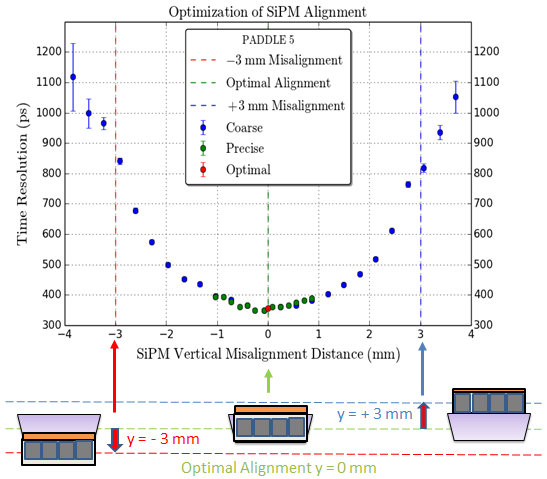
\includegraphics[width=1.0\columnwidth]{misalignment/figs/sipm_va_coarse}
%		\caption{Vertical misalignment results.  The minimum time resolution obtained was approximately 350 ps which was expected.  Once the SiPM exceeded $y = \pm 3\ mm$, no active area of the SiPM was directly coupled to the face of the scintillator.}
%		\label{fig:sipm_va_coarse}
%	\end{figure}
	\begin{figure}[!htb]
	\centering
	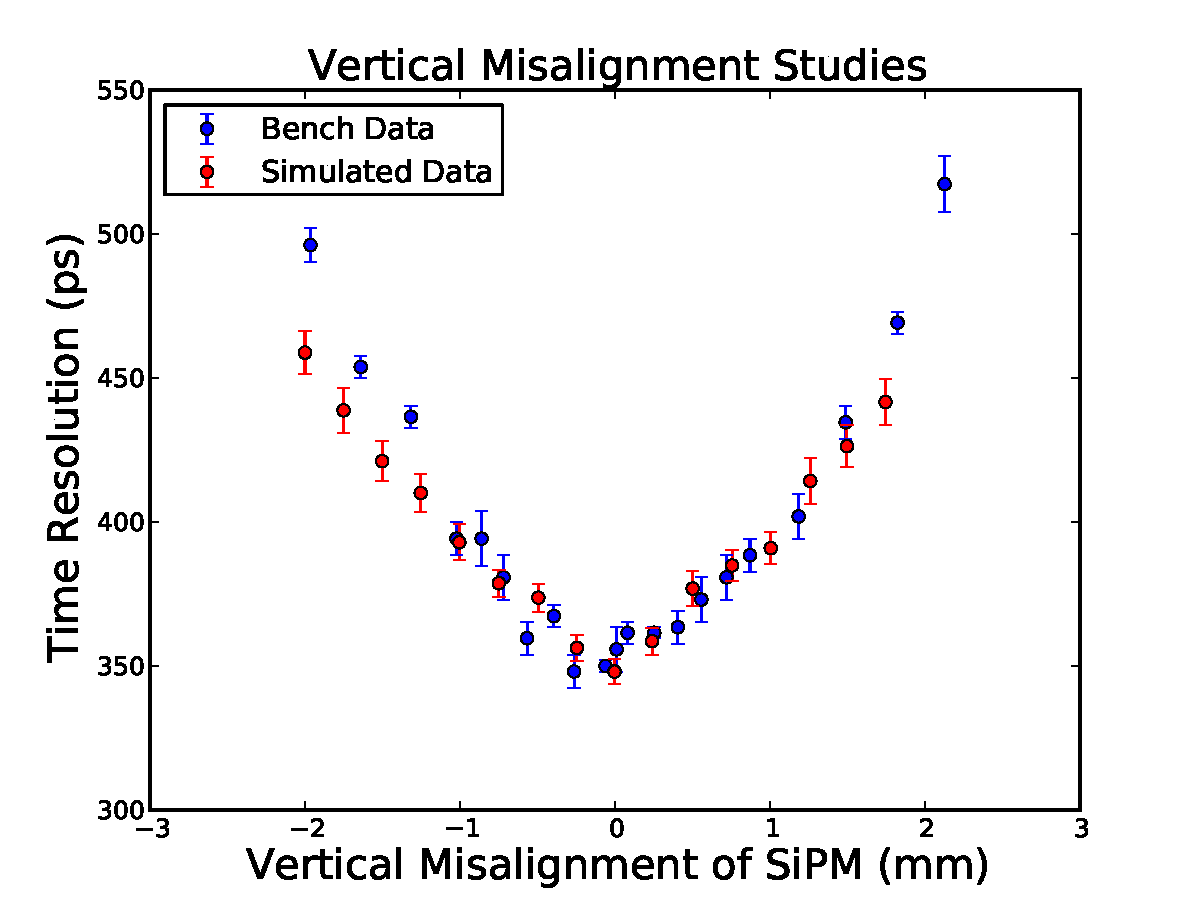
\includegraphics[width=1.0\columnwidth]{misalignment/figs/vert_ma}
	\caption{Vertical misalignment results.  The minimum time resolution obtained was approximately 350 ps which was expected.  Once the SiPM exceeded $y = \pm 3\ mm$, no active area of the SiPM was directly coupled to the face of the scintillator.}
	\label{fig:sipm_va}
\end{figure}
%For each distinct location of the SiPM, the distance traversed was verified by a manual measurement made with a micrometer with $25\ \mu m$ precision.
%From the vertical misalignment studies it is clear that there is no significant variation of time resolution within a $\pm 300\ \mathrm{\mu m}$ range of the optimal alignment.
The results indicate that there is no significant variation of time resolution within a $\pm 300\ \mathrm{\mu m}$ range of the optimal alignment.  

Vertical misalignments were also simulated in a manner similar to what was discussed in section \ref{sec:sim_mach} and the results are seen in Fig. \ref{fig:sipm_va}.
%	\begin{figure}[!htb]
%		\centering
%		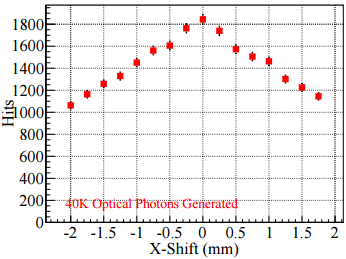
\includegraphics[width=0.8\columnwidth]{misalignment/figs/vertical_sim}
%		\caption{Vertical alignment simulation studies \cite{puneet_sim_talk}.}
%		\label{fig:vertical_sim}
%	\end{figure}
The GEANT4 simulations indicate that the acceptable range of vertical misalignment is approximately $\pm 250\ \mathrm{\mu m}$ \cite{puneet_sim_talk} which is consistent with what was measured on the bench.

\subsection{Coupling Distance of SiPM \& Scintillator}

With the vertical alignment between the scintillator and SiPM optimized, the effects of varying the coupling distance were also studied.  Using an identical set-up as was described in section \ref{sec:misalign_vert} the coupling distance, and resulting time resolutions, were measured at various locations along $z$ illustrated in Fig.~\ref{fig:sipm_va_optics}.  While the coupling distance was varied, the vertical alignment $y$ was kept constant at the optimal location \textit{i.e.} $y = 0$, and was monitored both optically and manually with a micrometer.
% WB skip thiso figure  
% EP done.
%	\begin{figure}[!htb]
%		\centering
%		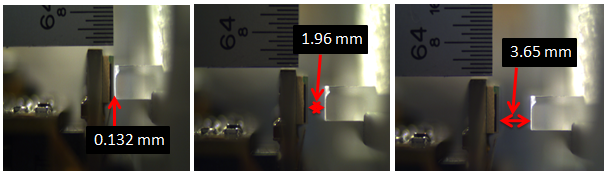
\includegraphics[width=1.0\columnwidth]{misalignment/figs/sipm_coupling_optics}
%		\caption{Various coupling distances as measured with the CMOS camera.  The high degree of precision is clearly visible.}
%		\label{fig:sipm_coupling_optics}
%	\end{figure}

%The SiPM was moved \textit{via} the MT translation stage along the $z-axis$.  We defined $z = 0$ to be the instance when the active area of the SiPM was flush against the face of the machined scintillator paddle.  In the coupling region $z < 1\ \mathrm{mm}$ the SiPM was receded from the face of the SiPM in 1/4 turn intervals ($79.5\ \mathrm{\mu m}$).  For $\mathrm{1\ mm < z < 2\ mm}$, the SiPM was receded from the face of the SiPM in 1/2 turn intervals ($159\ \mathrm{\mu m}$), and for $\mathrm{2\ mm < z < 4\ mm}$ data were collected in 1 turn intervals ($\mathrm{318\ \mu m}$) with the results being illustrated in Fig. \ref{fig:sipm_coupling_coarse}.
The SiPM was moved \textit{via} the MT translation stage along the $z-axis$.  We defined $z = 0$ to be the instance when the active area of the SiPM was flush against the face of the machined scintillator paddle.  Further details regarding the three coupling intervals shown in Fig. \ref{fig:sipm_coupling} are discussed further in Ref.~\cite{pooser16}.  The results of this study are illustrated in Fig. \ref{fig:sipm_coupling}.
%	\begin{figure}[!htb]
%		\centering
%		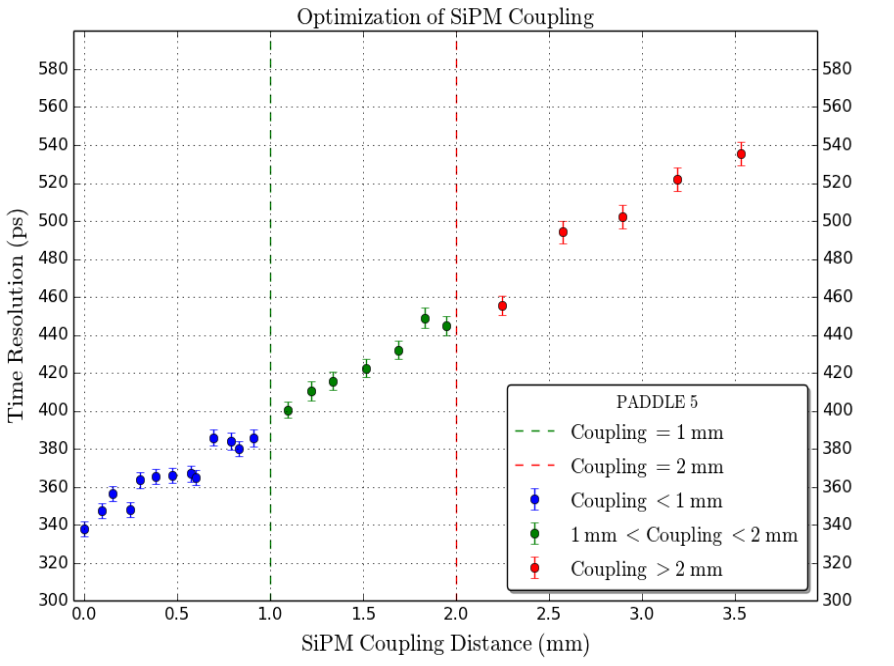
\includegraphics[width=0.83\columnwidth]{misalignment/figs/sipm_coupling_coarse}
%		\caption{Coupling distance studies.  It is useful to note that at a coupling distance of $\mathrm{251\ \mu m}$ the time resolution was identical to what was measured in Fig. \ref{fig:sipm_va} while conducting the vertical alignment studies.}
%		\label{fig:sipm_coupling_coarse}
%	\end{figure}
	\begin{figure}[!htb]
	\centering
	\includegraphics[width=1.0\columnwidth]{misalignment/figs/hori_ma}
	\caption{Coupling distance studies.  It is useful to note that at a coupling distance of $\mathrm{251\ \mu m}$ the time resolution was identical to what was measured in Fig. \ref{fig:sipm_va} while conducting the vertical alignment studies.}
	\label{fig:sipm_coupling}
	\end{figure}

The slight disagreement between bench data and simulation observed at large coupling distances ($\mathrm{> 1 mm}$) in the horizontal misalignment studies is attributed to a systematic error in which the active area of the SiPM was not parallel to the upstream end of the scintillator paddle during these measurements. It is clear from the data that the optimal coupling range was $\mathrm{50\ \mu m < z < 350\ \mu m}$ and there was no significant reduction in time resolution performance or light collection over a $\mathrm{0\ \mu m < z < 600\ \mu m}$ range.
%	\begin{figure}[!htb]
%		\centering
%		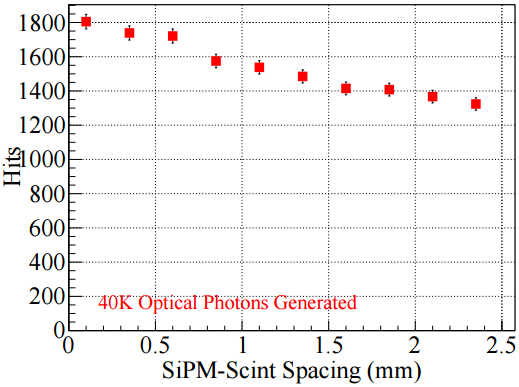
\includegraphics[width=0.8\columnwidth]{misalignment/figs/spacing_sim}
%		\caption{Coupling distance simulations. Simulations indicated that the optimal coupling distance is in the $50\ \mu m < z < 350\ \mu m$ range.}
%		\label{fig:spacing_sim}
%	\end{figure}